\documentclass[technicalreport]{ieicej}
\usepackage[dvipdfmx]{graphicx}
\usepackage[T1]{fontenc}
\usepackage{lmodern}
\usepackage{textcomp}
\usepackage{latexsym}
\usepackage{amsmath}
\usepackage{cite}
\usepackage{tikz}
\usepackage{geometry}
\usepackage{url}
\usepackage{schemabloc}
\usepackage{tikz}
\usetikzlibrary{arrows}

\usetikzlibrary{positioning,fit,calc}
\tikzset{block/.style={draw, thick, text width=1cm, minimum height=0.5cm, align=center}, line/.style={-latex}}  

\renewcommand{\figurename}{Fig.} % name the picture Fig.num
\renewcommand{\tablename}{Table } % name the table Table num
\renewcommand{\refname}{REFERENCE} % insert reference 

%调整文件显示位置和纸张
\geometry{
	a4paper,
	total={170mm,257mm},
	left=20mm,
	top=20mm,
}

\hoffset=-5mm
\voffset=-5mm

\def\IEICEJcls{\texttt{ieicej.cls}}
\def\IEICEJver{3.0}
\newcommand{\AmSLaTeX}{%
$\mathcal A$\lower.4ex\hbox{$\!\mathcal M\!$}$\mathcal S$-\LaTeX}
\def\BibTeX{{\rmfamily B\kern-.05em{\scshape i\kern-.025em b}\kern-.08em
T\kern-.1667em\lower.7ex\hbox{E}\kern-.125em X}}

\jtitle{M1課題レポート 第1回目}
\jsubtitle{}
\etitle{Technical Report for M1 Labwork 1-st}
\esubtitle{}
\authorlist{ % author name list
\authorentry[liuyuchen@radio.ict.e.titech.ac.jp]{りゅう ゆしん}{Yuchen Liu}{Titech}
}

\affiliate[Titech]{東京工業大学 〒152-8550 東京都目黒区大岡山2-12-1}
{Tokyo Institute of Technology,~~2-12-1, O-okayama, Meguro-ku, Tokyo, 152-8550 Japan}

\begin{document}

\begin{eabstract}
In this first C workshop, we will use C langaugae to simulate the workflow of a QPSK modulation and dection system over AWGN channel. In the begin, this report will introduce the overall design of the communicion system. Then the background knowlege is introduced. Final part is the simulation desgin come with simulation result compared to theoretical value.
\end{eabstract}

\maketitle

\section{Introduction}
QPSK is kind of digital phase shifting modulation method, which conveys data by changing the phase of a constant amplitude high freuqency carrier. Compared with BPSK, which can only use two phases, QPSK can utilize four phases, and one symbol is able to convey 2 bits of information. QPSK is widly deployed in system like wireless LANS, RFID, Bluetooth, etc. To map the bit to QPSK symbol, we aslo adopt gray code which is an ordering of the binary numeral system that two successive values differ in only one bit. Gray code is an effective strategy to improve total system performance.Corresponding bit mapping is in Table 1.\par
The channel we choose to conduct the simulation is AWGN, which is the simplest model to mimic the effect of many random process that occurs in nature due to thermal phenomenon. The  
expression formula is as followed:
\begin{equation}\label{1}
R(t)=S(t)+N
\end{equation}
$R(t)$ is received signal and $S(t)$ is transmitted signal, W is AWGN. The characteristic of AWGN is a normal ditribution in time domain, Guassian ditribution in amplitude and is able to directly add in original signal\cite{wiki:Additive_white_Gaussian_noise}.\par
In the receiver side, we use MLE as our estimation method to determine received symbol in constellation diagram\cite{kay1993fundamentals}. MLE is a method to estimate parameters of a probablity distribution by maximizing a likelihood function. The genral form of MLE is shown:
\begin{equation}\label{2}
 \hat{\theta}=\mathop{\arg\max}_{\theta\in\left ( \frac{\pi}{4},\frac{3\pi}{4},\frac{5\pi}{4},\frac{7\pi}{4}\right ) }\left \| R(t)-\theta_{i} \right \|
\end{equation}
In our caese, the likelihood function is the distance between received signal and constellation diagram.

\begin{table}[tbp]
	\begin{center}
	\caption{MAPPING TABLE OF PHASE}
	\begin{tabular}{ll}
	\hline
	\textbf{bitA bitB} & \textbf{$\Delta\theta_{i}$} \\
	\hline
	0 0 & $\frac{\pi}{4}$ \\
	1 0 & $\frac{3\pi}{4}$ \\
	1 1 & $\frac{5\pi}{4}$ \\
	1 0 & $\frac{7\pi}{4}$ \\
	\hline
	\end{tabular}
	\end{center}
\end{table}

\begin{table}[tbp]
	\begin{center}
	\caption{ACRONYMS AND FULL MEANING}
	\begin{tabular}{|l|l|}
	\hline
	\textbf{Acronyms} & \textbf{Full Form} \\
	\hline
	 MLE & Maximum Likelihood Estimator  \\ 
	 \hline
	 QPSK & Quadrature Phase Shift Keying  \\ 
	 \hline
	 SNR & Signal Noise Ratio \\ 
	 \hline
	 CNR & Channel Noise Ratio  \\ 
	 \hline
	 BPSK & Binary Phase Shift Keying  \\ 
	 \hline
	 AWGN & Additive White Gaussian Noise \\ 
	 \hline
	 BW & Band Width  \\ 
	 \hline
	\end{tabular}
	\end{center}
\end{table}

\begin{table}[hb]
	\begin{center}
	\caption{SIMULATION CONDITIONS}
	\label{tbl:simu}
	\small
	\begin{tabular}{ll}
	\hline
	ITEMS & CONDITIONS\\
	\hline
	Moduation Method & QPSK \\
	Transmission 	Bits & 128 \\
	Channel & AWGN \\
	Detection & MLE \\
	Number of Trials & $10^{6}$\\
	\hline
	\end{tabular}
	\end{center}
\end{table}

\section{Simulation and Result}
In our simulation, first we use C standard liabray rand() function to generate information bits, and then convert serial bit to 2 parallel bit and map the bit to QPSK symbol. To generate noise to simulate channel, we adopt Box-Muller method, the formula is shown:
\begin{equation}\label{3}
n_{k}=\sqrt{-\sigma^{2}_{n}\ln (u_{1})}e^{j2\pi u_{2}}
\end{equation}
In this equation, $u_{1}$ and $u_{2}$ are uniform distribution ranging from 0 to 1, which can be generated by C rand() function. The $\sigma^2_{n}$ is noise power which is:
\begin{equation}\label{4}
\sigma^{2}_{n}=10^{-\frac{CNR}{10}}
\end{equation}
$CNR$ in our cases is $SNR$ add 3 dB, because according to \cite{inproceedings}, modulation rotation gain of QPSK is 3 dB. Finally, we use the MEL mentioned earlier to estimation received signal and calculate BER.\par
In order to verify the validity of the Gray code, we run simulation on SNR from 0 to 11 dB in using gray code and without gray code two cases. The simulation parameter is shown in Table 3 and simulation result is in Figure 1. The BER of QPSK modulation over AWGN is shown as follow:
\begin{equation}\label{5}
\frac{1}{2}\rm erfc(\sqrt{\exp (SNR\cdot \frac{\ln 10}{10}))})
\end{equation}

\begin{figure}[tbp]
	\begin{center}
		\vspace{0cm}
		\includegraphics[width=\linewidth,clip]{fig/awgn.eps}
		\caption{QPSK BER IN DIFFERENT SNR}
		\label{fig:sample}
	\end{center}
\end{figure}

\section{Conclusion}
From Figure 2 we can see that the simulation result is very close to the theoretical value. And the BER curve withou gray code is obviously higher than deployed, this shows that Gray Code can effectively improve system performance.

\bibliographystyle{IEEEtran}
\bibliography{awgn.bib}

\end{document} 